% \begin{figure}
% % \begin{wrapfigure}{R}{0.5\textwidth}
% % 	\vspace{-20pt}
% 	\begin{center}
%     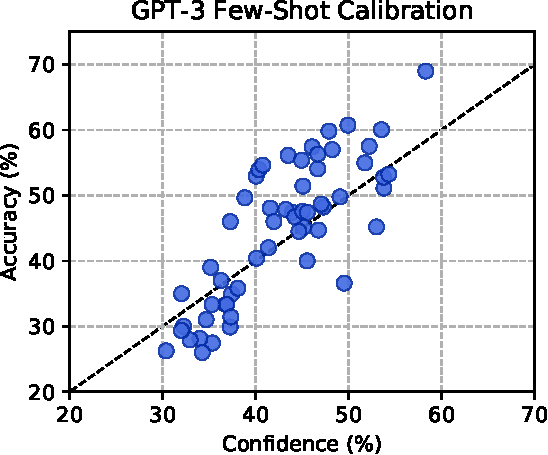
\includegraphics[width=0.5\textwidth]{figures/few_shot_calibration.pdf}
%     \caption{Few-shot calibration}\label{fig:fewshotcalibration}
%     \end{center}
% % 	\vspace{-20pt}
% \end{figure}
% % \end{wrapfigure}

\section{Additional Analysis}\label{app:additional}

% \begin{wrapfigure}{L}{0.5\textwidth}
% 	\vspace{-10pt}
% 	\begin{center}
% 	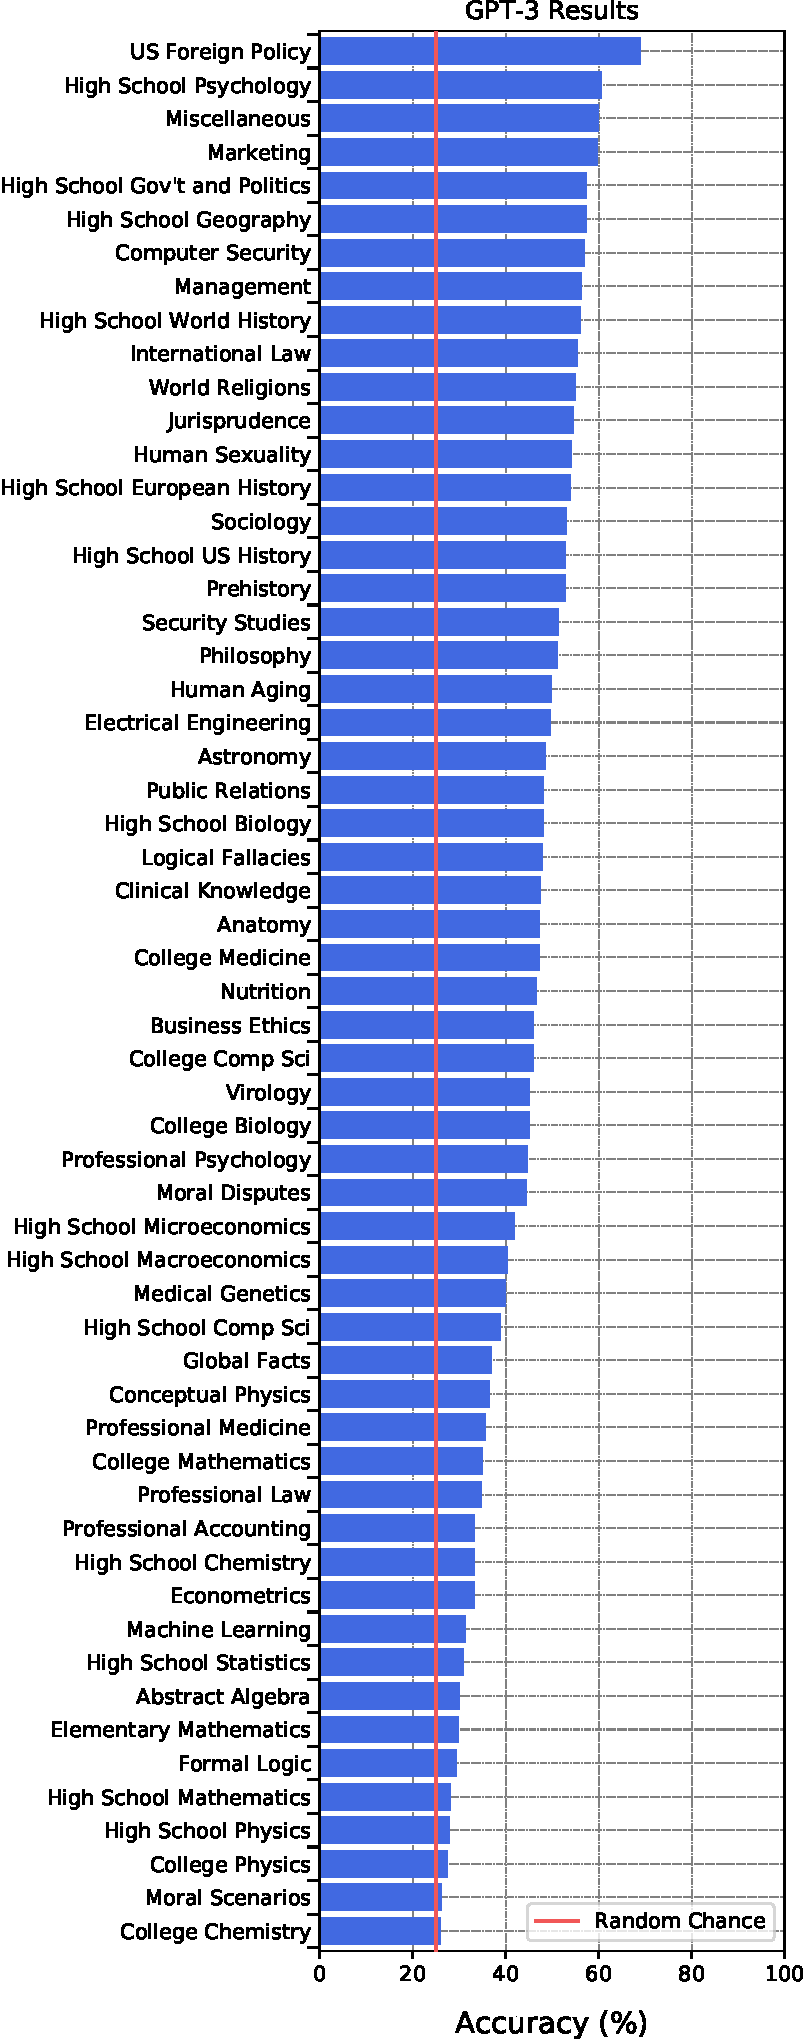
\includegraphics[width=0.5\textwidth]{figures/full_results.pdf}
% 	\end{center}
% 	\vspace{-10pt}
% 	\caption{GPT-3 few shot accuracies for all of the $57$ tasks. All task accuracies are markedly below expert-level performance.
%     }\label{fig:fullresults}
% 	\vspace{-20pt}
% \end{wrapfigure}

% \begin{wrapfigure}{R}{0.5\textwidth}
% 	\vspace{-18pt}
% 	\begin{center}
% 	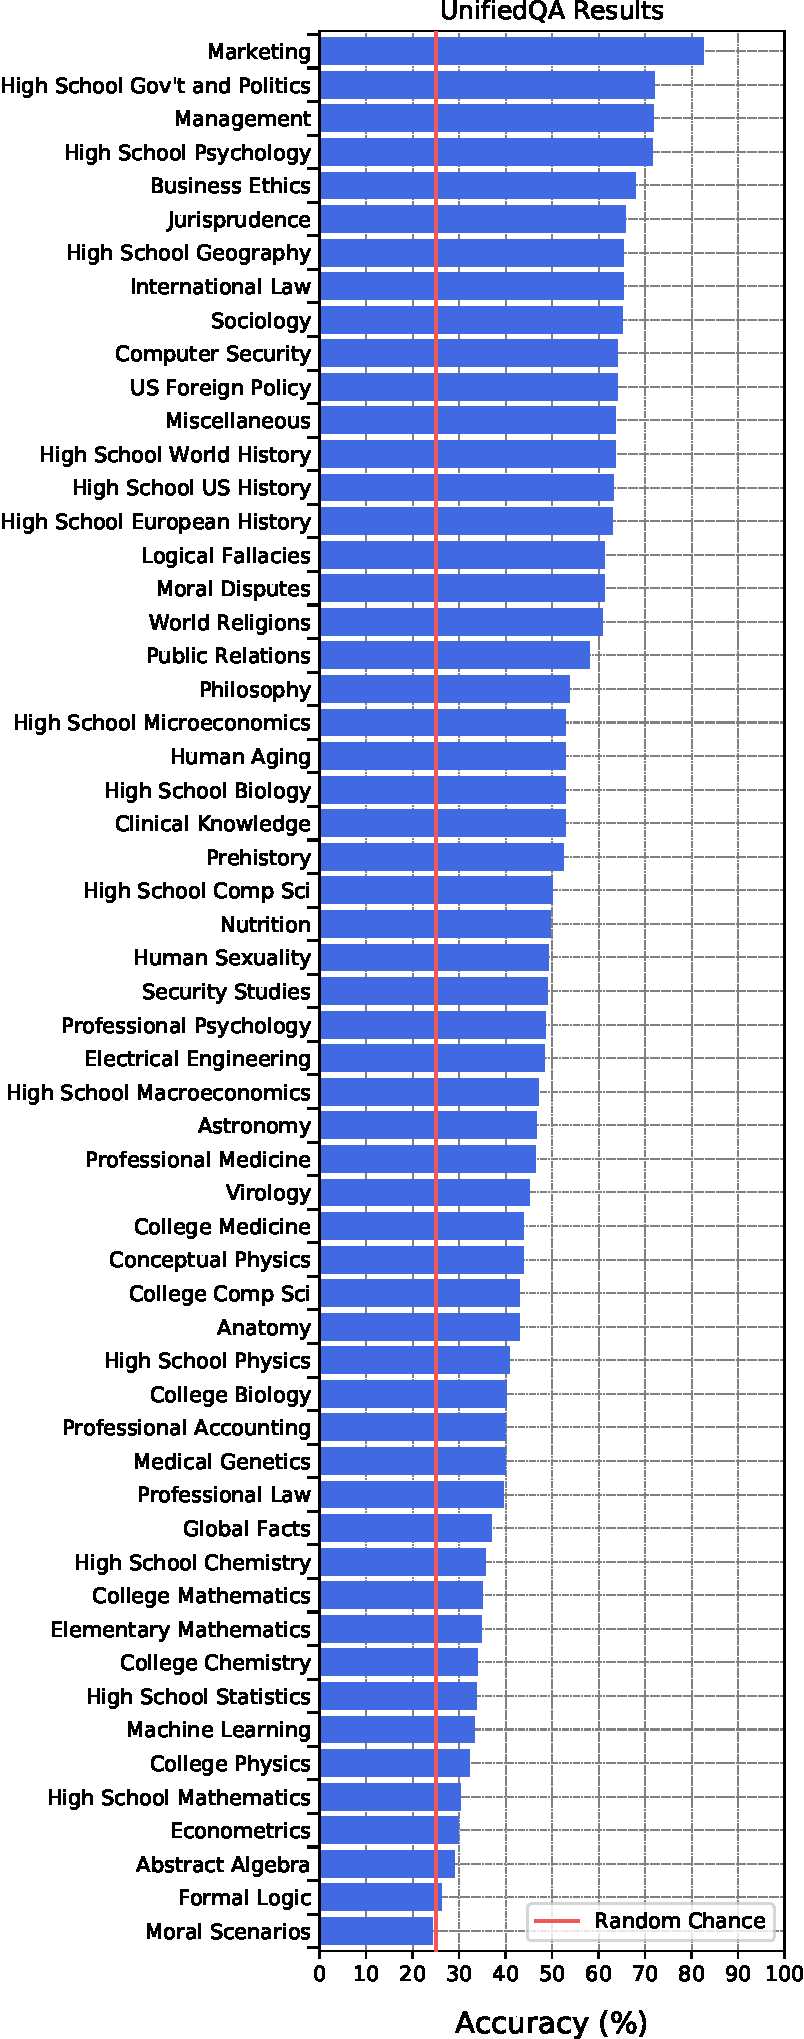
\includegraphics[width=0.5\textwidth]{figures/unifiedqa_results.pdf}
% 	\end{center}
% 	\vspace{-10pt}
% 	\caption{UnifiedQA accuracies for all of the $57$ tasks. Again, capabilities are lopsided.}\label{fig:unifiedqaresults}
% 	\vspace{-40pt}
% \end{wrapfigure}

This appendix includes figures with sorted results (\Cref{fig:unifiedqaresults}), few-shot examples vs. accuracy (\Cref{fig:kandacc}), and few-shot calibration (\Cref{fig:fewshotcalibration}). It also includes sections on fine-tuning, error analysis, and format sensitivity.

\begin{figure}[h]
% \vspace{-25pt}
\begin{subfigure}{.49\textwidth}
\centering
    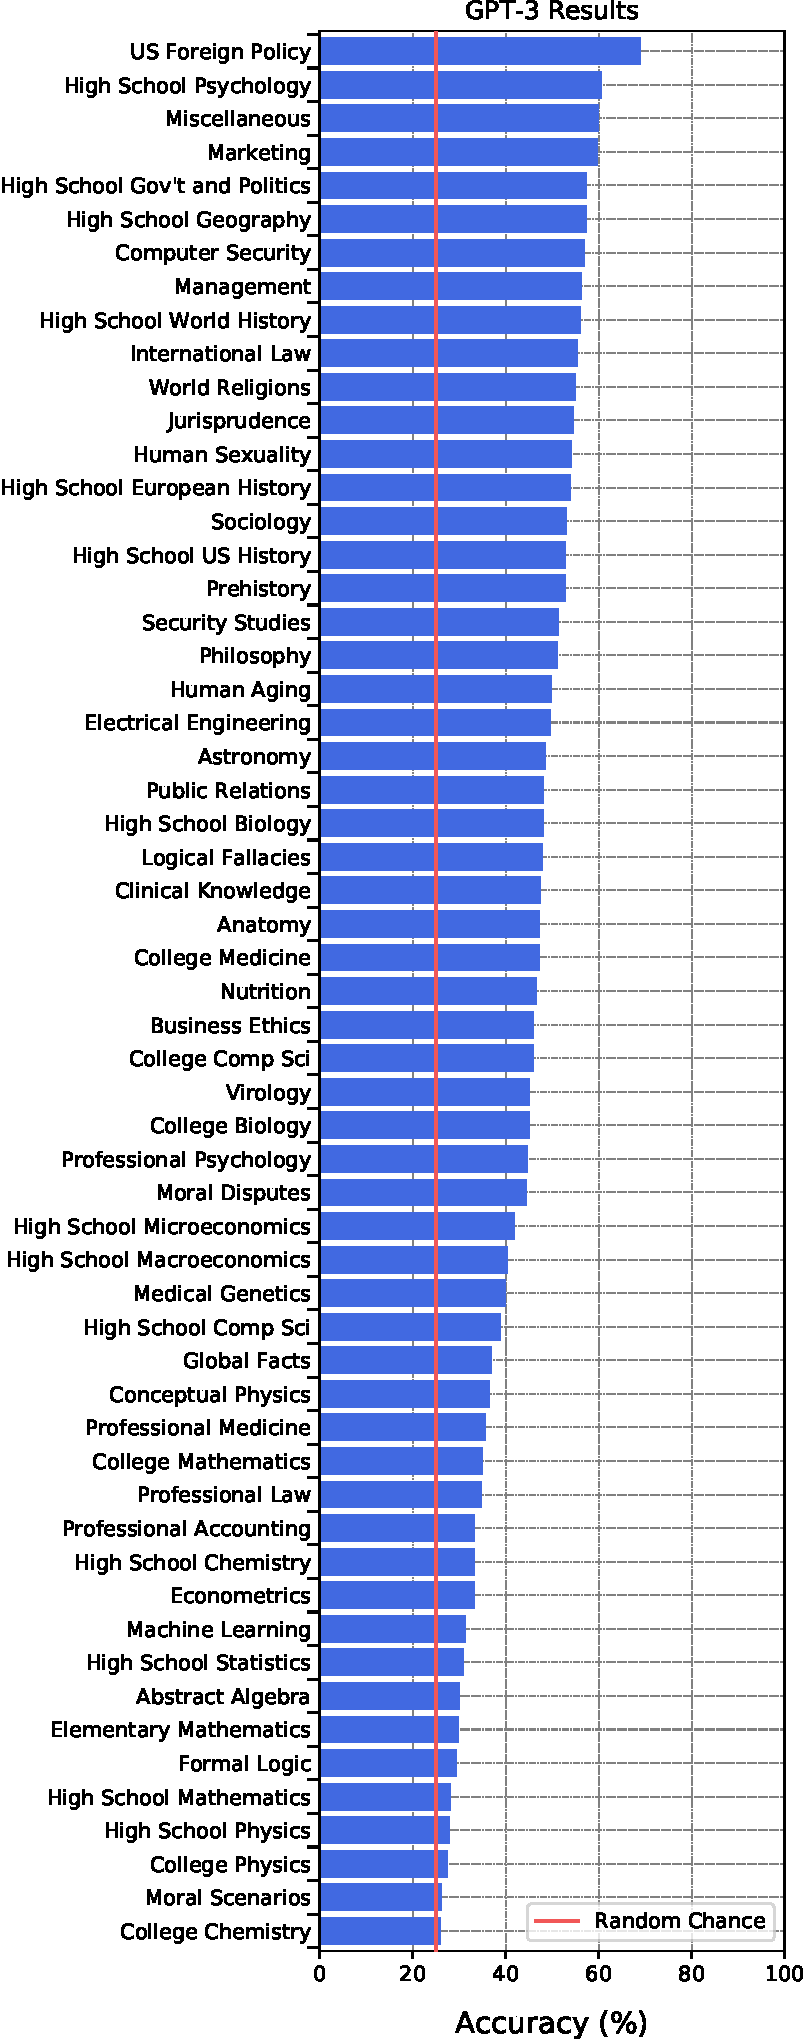
\includegraphics[width=\textwidth]{figures/full_results.pdf}
\end{subfigure}\hfill%
\begin{subfigure}{.49\textwidth}
\centering
    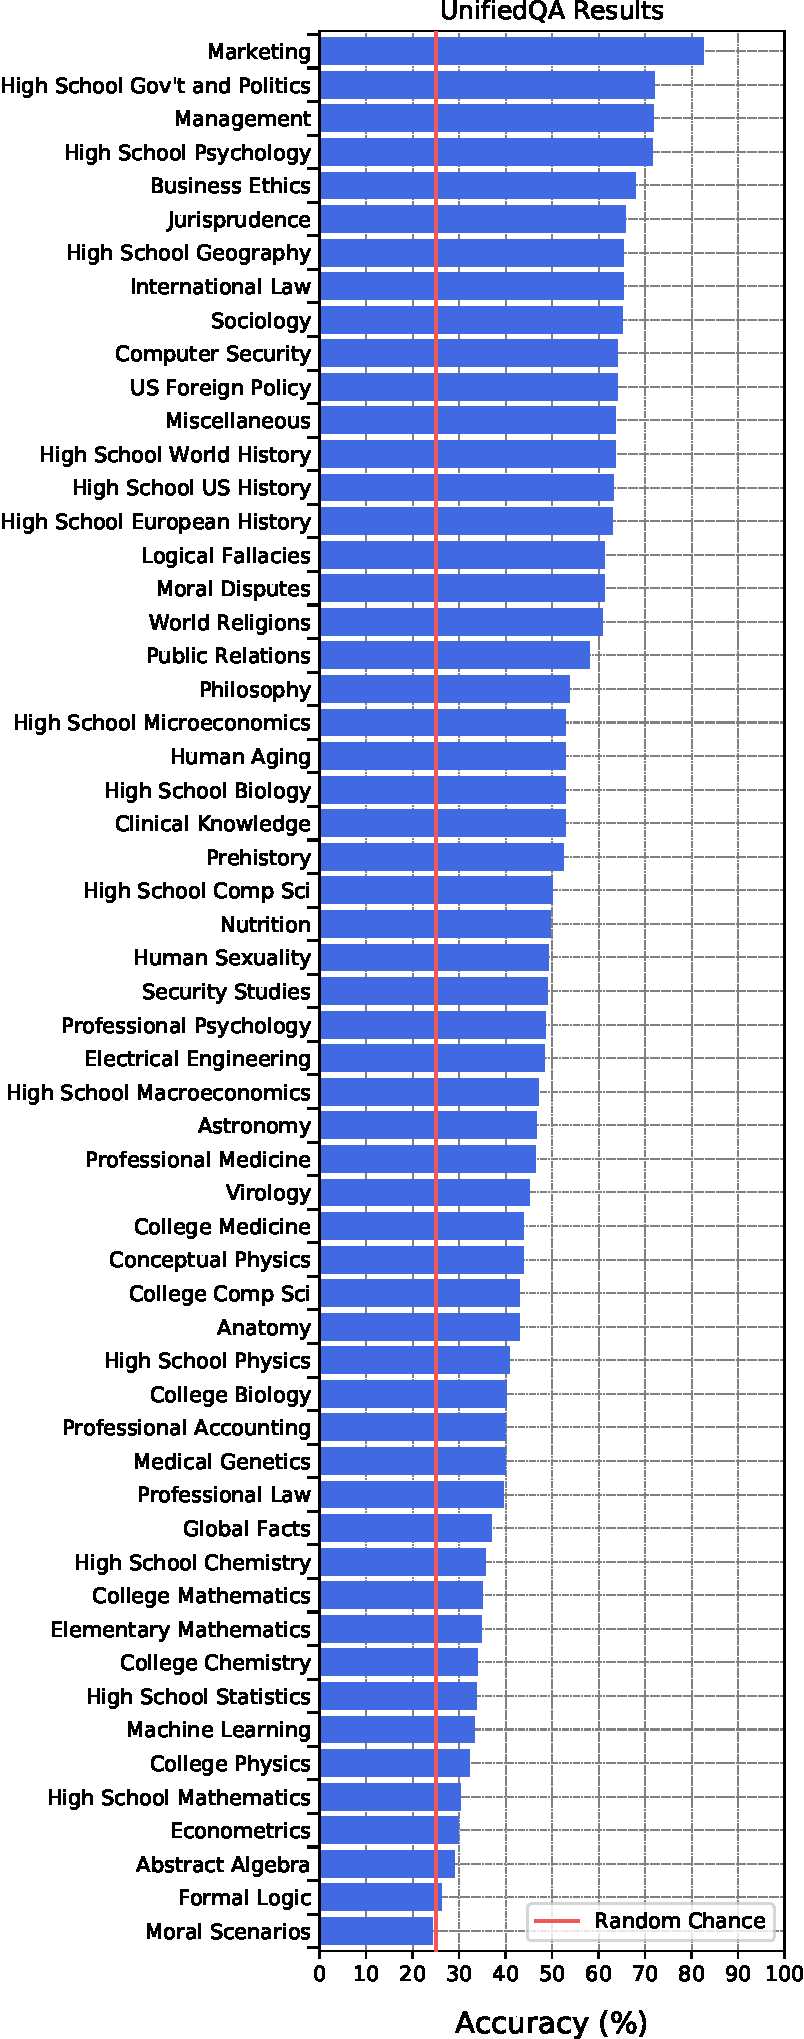
\includegraphics[width=\textwidth]{figures/unifiedqa_results.pdf}
\end{subfigure}
\caption{On the left are GPT-3 few shot accuracies for all of the $57$ tasks. On the right are UnifiedQA transfer accuracies for all of the $57$ tasks. For both models, capabilities are lopsided.}\label{fig:unifiedqaresults}
% \vspace{-13pt}
\end{figure}


\subsection{Analysis with More Fine-Tuned Models}
We primarily analyzed models with more than $10$ billion parameters in the main body of the paper. For this section, we analyze smaller models including RoBERTa-base (125 million parameters) \citep{RobertaLiu2019AR}, ALBERT-xxlarge (223 million parameters) \citep{AlbertLan2020}, and GPT-2 (1,558 million parameters) \citep{Radford2019LanguageMA}.
Models are fine-tuned to predict one of four classes using the UnifiedQA MCQ questions and using our dev+val set. We test on our multitask test set.

We observe that these smaller models can attain better-than-random accuracy. RoBERTa-base attains an overall accuracy of $27.9\%$, with $27.9\%$ accuracy for the humanities, $28.8\%$ for social sciences, $27.0\%$ for STEM, and $27.7\%$ for other. ALBERT-xxlarge attains an accuracy of $27.1\%$, with $27.2\%$ accuracy for the humanities, $25.7\%$ for the social sciences, $27.7\%$ for STEM, and $27.9\%$ for other. GPT-2 attains an accuracy of $32.4\%$, with $32.8\%$ accuracy for the humanities, $33.3\%$ for the social sciences, $30.2\%$ for STEM, and $33.1\%$ for other.

Compare this to UnifiedQA's smallest variant, which has just $60$ million parameters and approximately $29.3\%$ accuracy. It obtains higher accuracy than RoBERTa and ALBERT, even though it has fewer parameters. This suggests that its larger pretraining dataset enables higher accuracy. Likewise, UnifiedQA with $3$ billion parameters attains $43.7\%$, while the similarly sized GPT-2 model with $1.5$ billion parameters attains $32.4\%$ accuracy. This again suggests that T5's larger pretraining dataset size (and therefore UnifiedQA's pretraining dataset size) can increase accuracy.


% social sciences 33.1% 3099
% humanities 32.6% 4705
% other (business, health, misc.) 33.0% 3260
% STEM 29.9% 3015

\subsection{Error Analysis}
We qualitatively analyze when GPT-3 makes high confidence mistakes. We find that while many of these mistakes were clearly wrong, many were mistakes that a human might make. For example, one question it got wrong was ``How many chromosomes do all human somatic cells contain?'' The correct answer is $46$, while few-shot GPT-3 predicted $23$ with confidence $97.5\%$. This answer would have been correct if the question asked about the number of \emph{pairs} of chromosomes. Similarly, many of its other high confidence mistakes were also correct answers to slightly different questions.

\subsection{Format Sensitivity}
While different question formatting choices often lead to similar GPT-3 accuracies, we find that UnifiedQA is more sensitive.
UnifiedQA's input format is of the form
\begin{verbatim}
    QUESTION1 \\n (A) CHOICE1 (B) CHOICE2 (C) CHOICE3 (D) CHOICE4</s>
\end{verbatim}
where questions and choices are normalized and made lowercase.
If we remove the \texttt{</s>} from the input, accuracy declines by several percentage points.

\clearpage
\newpage

\begin{figure}[h]
% \vspace{-25pt}
\begin{minipage}{.49\textwidth}
\centering
    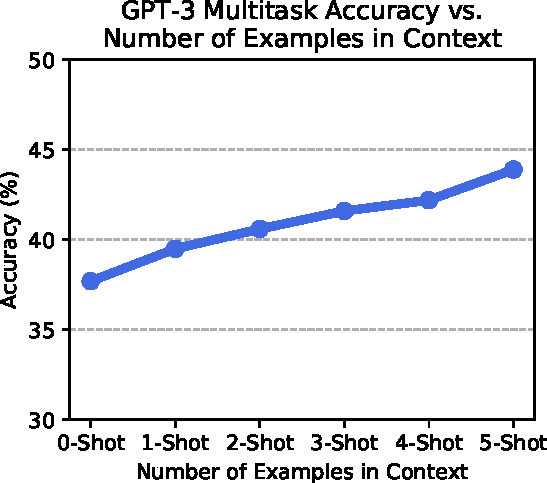
\includegraphics[width=\textwidth]{figures/shot_and_accuracy.pdf}
    \caption{As the number of few-shot instruction examples increases, the accuracy monotonically increases. Notably, zero-shot performance is only somewhat lower than $5$-shot accuracy.}\label{fig:kandacc}% Hence for this multitask test, additional prompt examples are only moderately effective at increasing accuracy and are not necessary to escape random-chance accuracy levels.\phantom{Here's some text to make sure the}}\label{fig:kandacc}
\end{minipage}\hfill%
\begin{minipage}{.49\textwidth}
\centering
    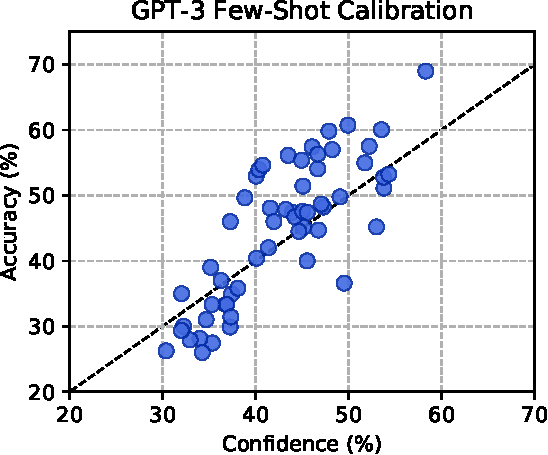
\includegraphics[width=\textwidth]{figures/few_shot_calibration.pdf}
    \caption{While models are more calibrated in a few-shot setting than a zero-shot setting, they are still miscalibrated, with gap between accuracy and confidence reaching up to $14\%$. Here the correlation between confidence and accuracy is $r=0.81$, compared to $r=0.63$ in the zero-shot setting.}\label{fig:fewshotcalibration}
\end{minipage}
% \vspace{-13pt}
\end{figure}



% RoBERTa-base (512) (Williams)
% Overall weighted acc: 27.9%

% Broad categories
% humanities 27.9% 4705
% social sciences 28.8% 3100
% STEM 27.0% 3015
% other (business, health, misc.) 27.7% 3260

% ALBERT
% Overall weighted acc: 27.1%

% Broad categories
% humanities 27.2% 4705
% social sciences 25.7% 3100
% STEM 27.7% 3015
% other (business, health, misc.) 27.9% 3260

% Question: {} (A) {} (B) {} (C) {} (D) {} Answer: {}\n
% Question: {} (A) {} (B) {} (C) {} (D) {} Answer: {}\n
% ...
% Question: {} (A) {} (B) {} (C) {} (D) {} Answer:
% Tried different prompts but this one was used.
% Used max length of 512 and 5-shot with cropping.
% I used the same evaluation procedures as Unifiedqa. Computed token overlap between 'model.generate(prompt)' and answer strings.
% give full unifiedqa results


%\dan{For each question, we choose the answer candidate with the highest token overlap of UnifiedQA’s generated text. When there is no exact match, we select the choice that produces the highest token overlap. In the case of ties, the answer was selected randomly among them.}


\section{Test Details}\label{app:fulllist}
\subsection{Task Descriptions and Examples}
We provide analysis of question length and difficulty in \Cref{fig:length}. We list all tasks and the topics they test in \Cref{tab:datasetdescriptions}. We also provide an example for each task starting with \Cref{fig:abstractalgebraexample}.


\begin{figure}[h]
% \vspace{-25pt}
\begin{subfigure}{.49\textwidth}
\centering
    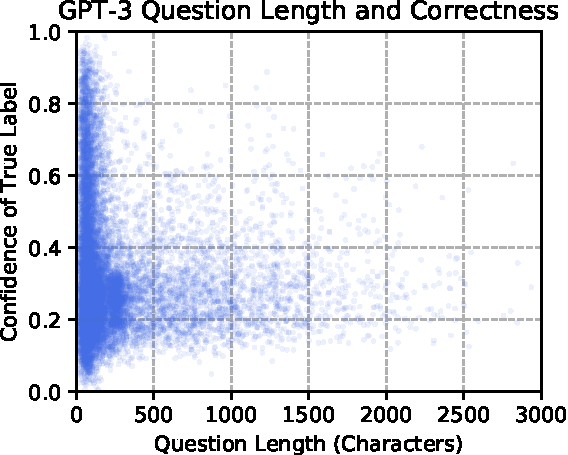
\includegraphics[width=\textwidth]{figures/question_length_v_acc.pdf}
\end{subfigure}\hfill%
\begin{subfigure}{.49\textwidth}
\centering
    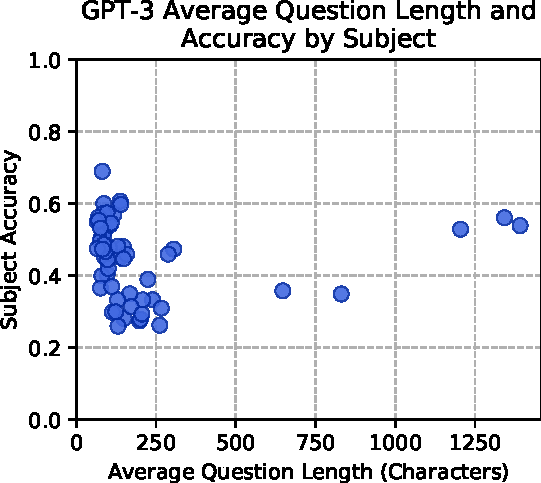
\includegraphics[width=\textwidth]{figures/subject_length_v_acc.pdf}
\end{subfigure}
\caption{Figures on the relation between question difficulty and question length.
For questions longer than a tweet (280 characters), the correlation between question length and true label confidence is slightly positive. This shows that longer questions are not necessarily harder.
}\label{fig:length}
% \vspace{-13pt}
\end{figure}

\subsection{Exact Question and Answer Contamination}
Since language models train on vast text corpora, there is some chance that they have seen the exact question and answer during pretraining. If they memorized the exact question and answer, then they would attain higher accuracy than their true ability. Likewise, a question's entropy would be especially low if it were memorized. Memorized questions and answers should have low entropy and high accuracy. However, in \Cref{fig:zeroshotnpt}, we see that accuracy and question entropy are not positively correlated, suggesting that the test's low-entropy questions do not correspond to memorized (and thereby correctly predicted) answers. This suggests that our \emph{exact} questions were not memorized. However, during pretraining models encountered text \emph{related} to our questions through processing Wikipedia. We also note that most of our questions came from PDFs or websites where questions and answers are on separate pages.

See \cite{brown2020gpt3} for a previous discussion of contamination showing that the phenomena hardly affects performance. To reduce the probability that future models encounter exact questions during test-time, we will provide a list of question sources.


\begin{figure}[h]
% \vspace{-25pt}
\begin{subfigure}{.49\textwidth}
\centering
    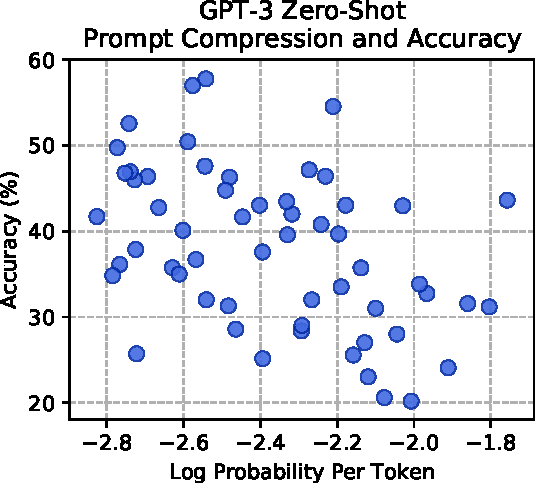
\includegraphics[width=\textwidth]{figures/zero_shot_npt.pdf}
\end{subfigure}\hfill%
\begin{subfigure}{.49\textwidth}
\centering
    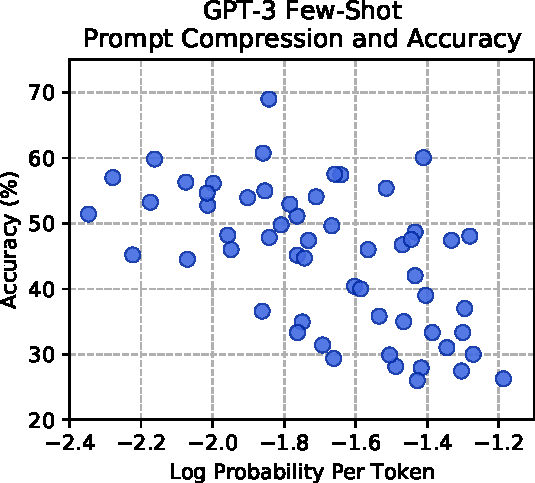
\includegraphics[width=\textwidth]{figures/few_shot_npt.pdf}
\end{subfigure}
\caption{The average log probability of the question (without answer) is not strongly positively correlated with accuracy, all else equal. Each point corresponds to a task. Higher log probability indicates higher compression, and especially high log probability would suggest memorization. In the zero-shot question prompt, the correlation between average log probability and accuracy is $r=-0.43$, and for the few-shot setting the correlation is $r=-0.56$.}\label{fig:zeroshotnpt}
% \vspace{-13pt}
\end{figure}




\begin{table}[h]
\setlength{\tabcolsep}{11pt}
% \vspace{-10pt}
%\scriptsize
% \footnotesize
\fontsize{10}{11}\selectfont
\centering
\noindent\makebox[\textwidth]{%
\begin{tabular}{lll}
Task       & Tested Concepts & Supercategory \\
\hline
Abstract Algebra & Groups, rings, fields, vector spaces, ... & STEM \\
Anatomy & Central nervous system, circulatory system, ...  & STEM \\
Astronomy & Solar system, galaxies, asteroids, ... & STEM \\
Business Ethics & Corporate responsibility, stakeholders, regulation, ...  & Other\\
Clinical Knowledge & Spot diagnosis, joints, abdominal examination, ... & Other \\
College Biology & Cellular structure, molecular biology, ecology, ... & STEM \\
College Chemistry & Analytical, organic, inorganic, physical, ... & STEM \\
College Computer Science & Algorithms, systems, graphs, recursion, ... & STEM \\
College Mathematics & Differential equations, real analysis, combinatorics, ... & STEM \\
College Medicine & Introductory biochemistry, sociology, reasoning, ... & Other \\
College Physics & Electromagnetism, thermodynamics, special relativity, ... & STEM \\
Computer Security & Cryptography, malware, side channels, fuzzing, ... & STEM \\
Conceptual Physics & Newton's laws, rotational motion, gravity, sound, ... & STEM \\
Econometrics & Volatility, long-run relationships, forecasting, ... & Social Sciences \\
Electrical Engineering & Circuits, power systems, electrical drives, ... & STEM \\
Elementary Mathematics & Word problems, multiplication, remainders, rounding, ... & STEM \\
Formal Logic & Propositions, predicate logic, first-order logic, ... & Humanities \\
Global Facts & Extreme poverty, literacy rates, life expectancy, ... & Other \\
High School Biology & Natural selection, heredity, cell cycle, Krebs cycle, ... & STEM \\
High School Chemistry & Chemical reactions, ions, acids and bases, ... & STEM \\
High School Computer Science & Arrays, conditionals, iteration, inheritance, ... & STEM \\
High School European History & Renaissance, reformation, industrialization, ... & Humanities \\
High School Geography & Population migration, rural land-use, urban processes, ... & Social Sciences \\
High School Gov't and Politics & Branches of government, civil liberties, political ideologies, ... & Social Sciences \\
High School Macroeconomics & Economic indicators, national income, international trade, ... & Social Sciences \\
High School Mathematics & Pre-algebra, algebra, trigonometry, calculus, ... & STEM \\
High School Microeconomics & Supply and demand, imperfect competition, market failure, ... & Social Sciences \\
High School Physics & Kinematics, energy, torque, fluid pressure, ... & STEM \\
High School Psychology & Behavior, personality, emotions, learning, ... & Social Sciences \\
High School Statistics & Random variables, sampling distributions, chi-square tests, ...  & STEM \\
High School US History & Civil War, the Great Depression, The Great Society, ... & Humanities \\
High School World History & Ottoman empire, economic imperialism, World War I, ... & Humanities \\
Human Aging & Senescence, dementia, longevity, personality changes, ... & Other \\
Human Sexuality & Pregnancy, sexual differentiation, sexual orientation, ... & Social Sciences \\
International Law & Human rights, sovereignty, law of the sea, use of force, ... & Humanities \\
Jurisprudence & Natural law, classical legal positivism, legal realism, ... & Humanities \\
Logical Fallacies & No true Scotsman, base rate fallacy, composition fallacy, ... & Humanities \\
Machine Learning & SVMs, VC dimension, deep learning architectures, ... & STEM \\
Management & Organizing, communication, organizational structure, ... & Other \\
Marketing & Segmentation, pricing, market research, ... & Other \\
Medical Genetics & Genes and cancer, common chromosome disorders, ... & Other \\
Miscellaneous & Agriculture, Fermi estimation, pop culture, ... & Other \\
Moral Disputes & Freedom of speech, addiction, the death penalty, ... & Humanities \\
Moral Scenarios & Detecting physical violence, stealing, externalities, ... & Humanities \\
Nutrition & Metabolism, water-soluble vitamins, diabetes, ... & Other \\
Philosophy & Skepticism, phronesis, skepticism, Singer's Drowning Child, ... & Humanities \\
Prehistory & Neanderthals, Mesoamerica, extinction, stone tools, ... & Humanities \\
Professional Accounting & Auditing, reporting, regulation, valuation, ... & Other \\
Professional Law &  Torts, criminal law, contracts, property, evidence, ... & Humanities \\
Professional Medicine & Diagnosis, pharmacotherapy, disease prevention, ... & Other \\
Professional Psychology & Diagnosis, biology and behavior, lifespan development, ... & Social Sciences \\
Public Relations & Media theory, crisis management, intelligence gathering, ... & Social Sciences \\
Security Studies & Environmental security, terrorism, weapons of mass destruction, ... & Social Sciences \\
Sociology & Socialization, cities and community, inequality and wealth, ... & Social Sciences \\
US Foreign Policy & Soft power, Cold War foreign policy, isolationism, ... & Social Sciences \\
Virology & Epidemiology, coronaviruses, retroviruses, herpesviruses, ... & Other \\
World Religions & Judaism, Christianity, Islam, Buddhism, Jainism, ... & Humanities\\
\hline
\end{tabular}}
% \vspace{2pt}
\caption{Summary of all $57$ tasks.}
\label{tab:datasetdescriptions}
% \label{results}
% \vspace{-10pt}
\end{table}


\clearpage
\begin{figure}
\centering
\fbox{\begin{minipage}{13.5 cm}
Find all $c$ in $\mathbb{Z}_3$ such that $\mathbb{Z}_3[x]/(x^2 + c)$ is a field.\\
(A) 0 \quad \textbf{(B) 1} \quad (C) 2 \quad (D) 3
\end{minipage}}
    \caption{An Abstract Algebra example.}
    \label{fig:abstractalgebraexample}
\end{figure}

\begin{figure}
\centering
\fbox{\begin{minipage}{13.5 cm}
What is the embryological origin of the hyoid bone?\\
(A) The first pharyngeal arch\\
(B) The first and second pharyngeal arches\\
(C) The second pharyngeal arch\\
\textbf{(D) The second and third pharyngeal arches}
\end{minipage}}
    \caption{An Anatomy example.}
    \label{fig:anatomyexample}
\end{figure}

\begin{figure}
\centering
\fbox{\begin{minipage}{13.5 cm}
Why isn't there a planet where the asteroid belt is located?\\
(A) A planet once formed here but it was broken apart by a catastrophic collision.\\
(B) There was not enough material in this part of the solar nebula to form a planet.\\
(C) There was too much rocky material to form a terrestrial planet but not enough gaseous material to form a jovian planet.\\
\textbf{(D) Resonance with Jupiter prevented material from collecting together to form a planet.}
\end{minipage}}
    \caption{An Astronomy example.}
    \label{fig:astronomyexample}
\end{figure}

\begin{figure}
\centering
\fbox{\begin{minipage}{13.5 cm}
Three contrasting tactics that CSO's can engage in to meet their aims are \underline{\hspace{1.5cm}} which typically involves research and communication, \underline{\hspace{1.5cm}}, which may involve physically attacking a company's operations or \underline{\hspace{1.5cm}}, often involving some form of \underline{\hspace{1.5cm}}.
\\
(A) Non-violent direct action, Violent direct action, Indirect action, Boycott\\
(B) Indirect action, Instrumental action, Non-violent direct action, Information campaign\\
\textbf{(C) Indirect action, Violent direct action, Non-violent direct-action Boycott.}\\
(D) Non-violent direct action, Instrumental action, Indirect action, Information campaign
\end{minipage}}
    \caption{A Business Ethics example.}
    \label{fig:businessethicsexample}
\end{figure}

\begin{figure}
\centering
\fbox{\begin{minipage}{13.5 cm}
How many attempts should you make to cannulate a patient before passing the job on to a senior colleague?\\
(A) 4 \quad (B) 3 \quad \textbf{(C) 2} \quad (D) 1
\end{minipage}}
    \caption{A Clinical Knowledge example.}
    \label{fig:clinicalknowledgeexample}
\end{figure}

\begin{figure}
\centering
\fbox{\begin{minipage}{13.5 cm}
In a given population, 1 out of every 400 people has a cancer caused by a completely recessive allele, b. Assuming the population is in Hardy-Weinberg equilibrium, which of the following is the expected proportion of individuals who carry the b allele but are not expected to develop the cancer?
\\
(A) 1/400 \quad (B) 19/400 \quad (C) 20/400 \quad \textbf{(D) 38/400}
\end{minipage}}
    \caption{A College Biology example.}
    \label{fig:collegebiologyexample}
\end{figure}

\begin{figure}
\centering
\fbox{\begin{minipage}{13.5 cm}
Which of the following statements about the lanthanide elements is NOT true?\\
(A) The most common oxidation state for the lanthanide elements is +3.\\
(B) Lanthanide complexes often have high coordination numbers (> 6).\\
(C) All of the lanthanide elements react with aqueous acid to liberate hydrogen.\\
\textbf{(D) The atomic radii of the lanthanide elements increase across the period from La to Lu.}
\end{minipage}}
    \caption{A College Chemistry example.}
    \label{fig:collegechemistryexample}
\end{figure}

\begin{figure}
\centering
\fbox{\begin{minipage}{13.5 cm}
Consider a computer design in which multiple processors, each with a private cache memory, share global memory using a single bus. This bus is the critical system resource. Each processor can execute one instruction every 500 nanoseconds as long as memory references are satisfied by its local cache. When a cache miss occurs, the processor is delayed for an additional 2,000 nanoseconds. During half of this additional delay, the bus is dedicated to serving the cache miss. During the other half, the processor cannot continue, but the bus is free to service requests from other processors. On average, each instruction requires 2 memory references. On average, cache misses occur on 1 percent of references. What proportion of the capacity of the bus would a single processor consume, ignoring delays due to competition from other processors?\\
(A) 1/50 \quad \textbf{(B) 1/27} \quad (C) 1/25 \quad (D) 2/27
\end{minipage}}
    \caption{A College Computer Science example.}
    \label{fig:collegecsexample}
\end{figure}


\begin{figure}
\centering
\fbox{\begin{minipage}{13.5 cm}
Let $A$ be a real $2\times2$ matrix. Which of the following statements must be true?\\
I. All of the entries of $A^2$ are nonnegative.\\
II. The determinant of $A^2$ is nonnegative.\\
III. If A has two distinct eigenvalues, then $A^2$ has two distinct eigenvalues.\\
(A) I only \quad \textbf{(B) II only} \quad (C) III only \quad (D) II and III only
\end{minipage}}
\caption{A College Mathematics example.}
\end{figure}


\begin{figure}
\centering
\fbox{\begin{minipage}{13.5 cm}
In a genetic test of a newborn, a rare genetic disorder is found that has X-linked recessive transmission. Which of the following statements is likely true regarding the pedigree of this disorder?\\
(A) All descendants on the maternal side will have the disorder.\\
(B) Females will be approximately twice as affected as males in this family.\\
\textbf{(C) All daughters of an affected male will be affected.}\\
(D) There will be equal distribution of males and females affected.
\end{minipage}}
\caption{A College Medicine example.}
\end{figure}

\begin{figure}
\centering
\fbox{\begin{minipage}{13.5 cm}
One end of a Nichrome wire of length 2L and cross-sectional area A is attached to an end of another Nichrome wire of length L and cross- sectional area 2A. If the free end of the longer wire is at an electric potential of 8.0 volts, and the free end of the shorter wire is at an electric potential of 1.0 volt, the potential at the junction of the two wires is most nearly equal to\\
\textbf{(A) 2.4 V}\\
(B) 3.3 V\\
(C) 4.5 V\\
(D) 5.7 V
\end{minipage}}
\caption{A College Physics example.}
\end{figure}

\begin{figure}
\centering
\fbox{\begin{minipage}{13.5 cm}
Why is it that anti-virus scanners would not have found an exploitation of Heartbleed?\\
(A) It's a vacuous question: Heartbleed only reads outside a buffer, so there is no possible exploit\\
(B) Anti-virus scanners tend to look for viruses and other malicious\\
(C) Heartbleed attacks the anti-virus scanner itself\\
\textbf{(D) Anti-virus scanners tend to look for viruses and other malicious code, but Heartbleed exploits steal secrets without injecting any code}
\end{minipage}}
\caption{A Computer Security example.}
\end{figure}

\begin{figure}
\centering
\fbox{\begin{minipage}{13.5 cm}
A model airplane flies slower when flying into the wind and faster with wind at its back. When launched at right angles to the wind, a cross wind, its groundspeed compared with flying in still air is\\
(A) the same \quad \textbf{(B) greater} \quad (C) less \quad (D) either greater or less depending on wind speed
\end{minipage}}
\caption{A Conceptual Physics example.}
\end{figure}


\begin{figure}
\centering
\fbox{\begin{minipage}{13.5 cm}
Consider the following AR(1) model with the disturbances having zero mean and unit variance\\
$y_t = 0.2 + 0.4 y_{t-1} + u_t$\\
The (unconditional) mean of $y$ will be given by\\
(A) 0.2 \quad (B) 0.4 \quad (C) 0.5 \quad \textbf{(D) 0.33}
\end{minipage}}
\caption{An Econometrics example.}
\end{figure}


\begin{figure}
\centering
\fbox{\begin{minipage}{13.5 cm}
A point pole has a strength of $4\pi \times 10^{-4}$ weber. The force in newtons on a point pole of $4\pi \times 1.5 \times 10^{-4}$ weber placed at a distance of 10 cm from it will be\\
\textbf{(A) 15 N.} \quad (B) 20 N. \quad (C) 7.5 N. \quad (D) 3.75 N.
\end{minipage}}
\caption{An Electrical Engineering example.}
\end{figure}


\begin{figure}
\centering
\fbox{\begin{minipage}{13.5 cm}
A total of 30 players will play basketball at a park. There will be exactly 5 players on each team. Which statement correctly explains how to find the number of teams needed?\\
(A) Add 5 to 30 to find 35 teams.\\
\textbf{(B) Divide 30 by 5 to find 6 teams.}\\
(C) Multiply 30 and 5 to find 150 teams.\\
(D) Subtract 5 from 30 to find 25 teams.
\end{minipage}}
\caption{An Elementary Mathematics example.}
\end{figure}


\begin{figure}
\centering
\fbox{\begin{minipage}{13.5 cm}
Determine whether the statements are logically equivalent or contradictory. If neither, determine whether they are consistent or inconsistent.\\
$E \supset (F \cdot E)$ and $\sim E \cdot F$\\
(A) Logically equivalent\\
(B) Contradictory\\
\textbf{(C) Neither logically equivalent nor contradictory, but consistent}\\
(D) Inconsistent
\end{minipage}}
\caption{A Formal Logic example.}
\end{figure}


\begin{figure}
\centering
\fbox{\begin{minipage}{13.5 cm}
As of 2017, how many of the world’s 1-year-old children today have been vaccinated against some disease?\\
\textbf{(A) 80\%}\\
(B) 60\%\\
(C) 40\%\\
(D) 20\%
\end{minipage}}
\caption{A Global Facts example.}
\end{figure}


\begin{figure}
\centering
\fbox{\begin{minipage}{13.5 cm}
Homologous structures are often cited as evidence for the process of natural selection. All of the following are examples of homologous structures EXCEPT\\
(A) the wings of a bird and the wings of a bat \\
(B) the flippers of a whale and the arms of a man\\
(C) the pectoral fins of a porpoise and the flippers of a seal\\
\textbf{(D) the forelegs of an insect and the forelimbs of a dog}
\end{minipage}}
\caption{A High School Biology example.}
\end{figure}


\begin{figure}
\centering
\fbox{\begin{minipage}{13.5 cm}
From the solubility rules, which of the following is true?\\
(A) All chlorides, bromides, and iodides are soluble\\
(B) All sulfates are soluble\\
(C) All hydroxides are soluble\\
\textbf{(D) All ammonium-containing compounds are soluble}
\end{minipage}}
\caption{A High School Chemistry example.}
\end{figure}


\begin{figure}
\centering
\fbox{\begin{minipage}{13.5 cm}
A list of numbers has n elements, indexed from 1 to n. The following algorithm is intended to display the number of elements in the list that have a value greater than 100. The algorithm uses the variables count and position. Steps 3 and 4 are missing.\\
 Step 1: Set count to 0 and position to 1.\\
 Step 2: If the value of the element at index position is greater\\
 than 100, increase the value of count by 1.\\
 Step 3: (missing step)\\
 Step 4: (missing step)\\
 Step 5: Display the value of count.\\
Which of the following could be used to replace steps 3 and 4 so that the algorithm works as intended?\\
(A) Step 3: Increase the value of position by 1.\\
Step 4: Repeat steps 2 and 3 until the value of count is greater than 100.\\
(B) Step 3: Increase the value of position by 1.\\
Step 4: Repeat steps 2 and 3 until t he value of position is greater than n.\\
(C) Step 3: Repeat step 2 until the value of count is greater than 100.\\
Step 4: Increase the value of position by 1.\\
\textbf{(D) Step 3: Repeat step 2 until the value of position is greater than n.\\
Step 4: Increase the value of count by 1.}
\end{minipage}}
\caption{A High School Computer Science example.}
\end{figure}


\begin{figure}
\centering
\fbox{\begin{minipage}{13.5 cm}
This question refers to the following information.\\
Albeit the king's Majesty justly and rightfully is and ought to be the supreme head of the Church of England, and so is recognized by the clergy of this realm in their convocations, yet nevertheless, for corroboration and confirmation thereof, and for increase of virtue in Christ's religion within this realm of England, and to repress and extirpate all errors, heresies, and other enormities and abuses heretofore used in the same, be it enacted, by authority of this present Parliament, that the king, our sovereign lord, his heirs and successors, kings of this realm, shall be taken, accepted, and reputed the only supreme head in earth of the Church of England, called Anglicans Ecclesia; and shall have and enjoy, annexed and united to the imperial crown of this realm, as well the title and style thereof, as all honors, dignities, preeminences, jurisdictions, privileges, authorities, immunities, profits, and commodities to the said dignity of the supreme head of the same Church belonging and appertaining; and that our said sovereign lord, his heirs and successors, kings of this realm, shall have full power and authority from time to time to visit, repress, redress, record, order, correct, restrain, and amend all such errors, heresies, abuses, offenses, contempts, and enormities, whatsoever they be, which by any manner of spiritual authority or jurisdiction ought or may lawfully be reformed, repressed, ordered, redressed, corrected, restrained, or amended, most to the pleasure of Almighty God, the increase of virtue in Christ's religion, and for the conservation of the peace, unity, and tranquility of this realm; any usage, foreign land, foreign authority, prescription, or any other thing or things to the contrary hereof notwithstanding.\\
English Parliament, Act of Supremacy, 1534\\
From the passage, one may infer that the English Parliament wished to argue that the Act of Supremacy would\\
(A) give the English king a new position of authority\\
(B) give the position of head of the Church of England to Henry VIII alone and exclude his heirs\\
(C) establish Calvinism as the one true theology in England\\
\textbf{(D) end various forms of corruption plaguing the Church in England}
\end{minipage}}
\caption{A High School European History example.}
\end{figure}


\begin{figure}
\centering
\fbox{\begin{minipage}{13.5 cm}
During the third stage of the demographic transition model, which of the following is true?\\
(A) Birth rates increase and population growth rate is less rapid.\\
\textbf{(B) Birth rates decline and population growth rate is less rapid.}\\
(C) Birth rates increase and population growth rate increases.\\
(D) Birth rates decrease and population growth rate increases.
\end{minipage}}
\caption{A High School Geography example.}
\end{figure}

\begin{figure}
\centering
\fbox{\begin{minipage}{13.5 cm}
Which of the following best states an argument made by James Madison in The Federalist number 10?\\
(A) Honest politicians can prevent factions from developing.\\
(B) Factions are more likely to occur in large republics than in small ones.\\
\textbf{(C) The negative effects of factionalism can be reduced by a republican government.}\\
(D) Free elections are the people's best defense against factionalism.
\end{minipage}}
\caption{A High School Government and Politics example.}
\end{figure}


\begin{figure}
\centering
\fbox{\begin{minipage}{13.5 cm}
Which of the following is not included in the U.S. GDP?\\
(A) The U.S. military opens a new base in a foreign country with 1000 U.S. personnel.\\
(B) Japanese consumers buy thousands of CDs produced in the United States.\\
\textbf{(C) An American pop singer performs a sold-out concert in Paris.}\\
(D) A French theatrical production tours dozens of American cities.
\end{minipage}}
\caption{A High School Macroeconomics example.}
\end{figure}


\begin{figure}
\centering
\fbox{\begin{minipage}{13.5 cm}
Joe was in charge of lights for a dance. The red light blinks every two seconds, the yellow light every three seconds, and the blue light every five seconds. If we include the very beginning and very end of the dance, how many times during a seven minute dance will all the lights come on at the same time? (Assume that all three lights blink simultaneously at the very beginning of the dance.)\\
(A) 3\\
\textbf{(B) 15}\\
(C) 6\\
(D) 5
\end{minipage}}
\caption{A High School Mathematics example.}
\end{figure}

\begin{figure}
\centering
\fbox{\begin{minipage}{13.5 cm}
If the government subsidizes producers in a perfectly competitive market, then\\
(A) the demand for the product will increase\\
(B) the demand for the product will decrease\\
\textbf{(C) the consumer surplus will increase}\\
(D) the consumer surplus will decrease
\end{minipage}}
\caption{A High School Microeconomics example.}
\end{figure}


\begin{figure}
\centering
\fbox{\begin{minipage}{13.5 cm}
A point charge, Q = +1 mC, is fixed at the origin. How much work is required to move a charge, Q = +8 µC, from the point (0, 4 meters) to the point (3 meters, 0)?\\
(A) 3.5 J\\
\textbf{(B) 6.0 J}\\
(C) 22.5 J\\
(D) 40 J
\end{minipage}}
\caption{A High School Physics example.}
\end{figure}

\begin{figure}
\centering
\fbox{\begin{minipage}{13.5 cm}
While swimming in the ocean, Ivan is frightened by a dark shadow in the water even before he has the chance to identify what the shadow is. The synaptic connections taking place during this incident of fright are best described by which of the following?\\
\textbf{(A) Messages are sent from the thalamus directly to the amygdala.}\\
(B) Messages are sent from the thalamus to the ``what'' and ``where'' pathways.\\
(C) Messages are sent from the parasympathetic nervous system to the cerebral cortex.\\
(D) Messages are sent from the frontal lobes to the pituitary gland.
\end{minipage}}
\caption{A High School Psychology example.}
\end{figure}


\begin{figure}
\centering
\fbox{\begin{minipage}{13.5 cm}
Jonathan obtained a score of 80 on a statistics exam, placing him at the 90th percentile. Suppose five points are added to everyone's score. Jonathan's new score will be at the\\
(A) 80th percentile.\\
(B) 85th percentile.\\
\textbf{(C) 90th percentile.}\\
(D) 95th percentile.
\end{minipage}}
\caption{A High School Statistics example.}
\end{figure}

\begin{figure}
\centering
\fbox{\begin{minipage}{13.5 cm}
This question refers to the following information.\\
``Society in every state is a blessing, but government even in its best state is but a necessary evil; in its worst state an intolerable one; for when we suffer, or are exposed to the same miseries by a government, which we might expect in a country without government, our calamity is heightened by reflecting that we furnish the means by which we suffer. Government, like dress, is the badge of lost innocence; the palaces of kings are built on the ruins of the bowers of paradise. For were the impulses of conscience clear, uniform, and irresistibly obeyed, man would need no other lawgiver; but that not being the case, he finds it necessary to surrender up a part of his property to furnish means for the protection of the rest; and this he is induced to do by the same prudence which in every other case advises him out of two evils to choose the least. Wherefore, security being the true design and end of government, it unanswerably follows that whatever form thereof appears most likely to ensure it to us, with the least expense and greatest benefit, is preferable to all others.''\\
Thomas Paine, Common Sense, 1776\\
Which of the following ``miseries'' alluded to above were most condemned by Anti-Federalists of the post-Revolutionary era?\\
(A) Organized response to Bacon's Rebellion.\\
(B) Federal response to Shays's Rebellion.\\
\textbf{(C) Federal response to the Whiskey Rebellion.}\\
(D) Federal response to Pontiac's Rebellion.
\end{minipage}}
\caption{A High School US History example.}
\end{figure}

\begin{figure}
\centering
\fbox{\begin{minipage}{13.5 cm}
This question refers to the following information.\\
``The real grievance of the worker is the insecurity of his existence; he is not sure that he will always have work, he is not sure that he will always be healthy, and he foresees that he will one day be old and unfit to work. If he falls into poverty, even if only through a prolonged illness, he is then completely helpless, left to his own devices, and society does not currently recognize any real obligation towards him beyond the usual help for the poor, even if he has been working all the time ever so faithfully and diligently. The usual help for the poor, however, leaves a lot to be desired, especially in large cities, where it is very much worse than in the country.''\\
Otto von Bismarck, 1884\\
Otto von Bismarck likely made this speech in reaction to which of the following issues?\\
(A) Social acceptance of child labor.\\
(B) Declining life expectancy in Germany.\\
\textbf{(C) Criticisms of German trade tariffs.}\\
(D) Negative effects attributed to industrial capitalism.
\end{minipage}}
\caption{A High School World History example.}
\end{figure}

\begin{figure}
\centering
\fbox{\begin{minipage}{13.5 cm}
All other things being equal, which of the following persons is more likely to show osteoporosis?\\
(A) An older Hispanic American woman\\
(B) An older African American woman\\
\textbf{(C) An older Asian American woman}\\
(D) An older Native American woman
\end{minipage}}
\caption{A Human Aging example.}
\end{figure}

\begin{figure}
\centering
\fbox{\begin{minipage}{13.5 cm}
Morning sickness is typically a problem:\\
\textbf{(A) during the first trimester}\\
(B) during the second trimester\\
(C) during the third trimester\\
(D) all through the pregnancy
\end{minipage}}
\caption{A Human Sexuality example.}
\end{figure}

\begin{figure}
\centering
\fbox{\begin{minipage}{13.5 cm}
Would a reservation to the definition of torture in the ICCPR be acceptable in contemporary practice?\\
(A) This is an acceptable reservation if the reserving country's legislation employs a different definition\\
\textbf{(B) This is an unacceptable reservation because it contravenes the object and purpose of the ICCPR}\\
(C) This is an unacceptable reservation because the definition of torture in the ICCPR is consistent with customary international law\\
(D) This is an acceptable reservation because under general international law States have the right to enter reservations to treaties
\end{minipage}}
\caption{An International Law example.}
\end{figure}

\begin{figure}
\centering
\fbox{\begin{minipage}{13.5 cm}
Which position does Rawls claim is the least likely to be adopted by the POP (people in the original position)?\\
\textbf{(A) The POP would choose equality above liberty.}\\
(B) The POP would opt for the `maximin' strategy.\\
(C) The POP would opt for the `difference principle.'\\
(D) The POP would reject the `system of natural liberty.'
\end{minipage}}
\caption{A Jurisprudence example.}
\end{figure}

\begin{figure}
\centering
\fbox{\begin{minipage}{13.5 cm}
John Stuart Mill: Each person's happiness is a good to that person, and the general happiness, therefore, a good to the aggregate of all persons.\\
\textbf{(A) Fallacy of Composition}\\
(B) Fallacy of Division\\
(C) Gambler's Fallacy\\
(D) Equivocation
\end{minipage}}
\caption{A Logical Fallacies example.}
\end{figure}

\begin{figure}
\centering
\fbox{\begin{minipage}{13.5 cm}
A 6-sided die is rolled 15 times and the results are: side 1 comes up 0 times; side 2: 1 time; side 3: 2 times; side 4: 3 times; side 5: 4 times; side 6: 5 times. Based on these results, what is the probability of side 3 coming up when using Add-1 Smoothing?\\
(A) 2/15 \quad \textbf{(B) 1/7} \quad (C) 3/16 \quad (D) 1/5
\end{minipage}}
\caption{A Machine Learning example.}
\end{figure}

\begin{figure}
\centering
\fbox{\begin{minipage}{13.5 cm}
According to Lewin, Lippet and White's 1939 experiment, which form of leadership produced the most work from participants?\\
(A) Laissez-faire\\
(B) Democratic\\
\textbf{(C) Authoritarian}\\
(D) A mix of laissez-faire and democratic
\end{minipage}}
\caption{A Management example.}
\end{figure}


\begin{figure}
\centering
\fbox{\begin{minipage}{13.5 cm}
The single group within society that is most vulnerable to reference group influence is:\\
(A) The older consumer who feels somewhat left out of things.\\
(B) The married women, many of whom feel a need for stability in their lives.\\
(C) New immigrants who really want to assimilate into their new culture.\\
\textbf{(D) Children, who base most of their buying decisions on outside influences.}
\end{minipage}}
\caption{A Marketing example.}
\end{figure}

\begin{figure}
\centering
\fbox{\begin{minipage}{13.5 cm}
Which of the following conditions does not show multifactorial inheritance?\\
(A) Pyloric stenosis\\
(B) Schizophrenia\\
(C) Spina bifida (neural tube defects)\\
\textbf{(D) Marfan syndrome}
\end{minipage}}
\caption{A Medical Genetics example.}
\end{figure}

\begin{figure}
\centering
\fbox{\begin{minipage}{13.5 cm}
If each of the following meals provides the same number of calories, which meal requires the most land to produce the food?\\
(A) Red beans and rice\\
\textbf{(B) Steak and a baked potato}\\
(C) Corn tortilla and refried beans	\\
(D) Lentil soup and brown bread	
\end{minipage}}
\caption{A Miscellaneous example.}
\end{figure}

\begin{figure}
\centering
\fbox{\begin{minipage}{13.5 cm}
In response to Sandel's ``social justice'' argument, Kamm argues that\\
(A) even if we were able to enhance ourselves or others, we would not thereby be obligated to do so.\\
(B) there is a difference between (i) choosing that one have a certain trait and (ii) being responsible for bearing the costs of that choice.\\
(C) having the option to enhance will lead to fewer instances of people who require the assistance of others.\\
\textbf{(D) all of the above}
\end{minipage}}
\caption{A Moral Disputes example.}
\end{figure}

\begin{figure}
\centering
\fbox{\begin{minipage}{13.5 cm}
For which of these two scenarios does the main character (who uses I/me/my) do something clearly morally wrong?\\
Scenario 1 | I drive very fast when I'm on a racetrack.\\
Scenario 2 | I drive very fast when I'm in the suburbs.\\
(A) Wrong, Wrong \\
(B) Wrong, Not wrong \\
\textbf{(C) Not wrong, Wrong}\\
(D) Not wrong, Not wrong
\end{minipage}}
\caption{A Moral Scenarios example. The formatting of this task hinders UnifiedQA performance substantially.}
\end{figure}

\begin{figure}
\centering
\fbox{\begin{minipage}{13.5 cm}
Which of the following is the most plausible explanation for the protective effect of dietary fibre against cancer of the colon?\\
(A) Propionic acid, formed during colonic fibre fermentation inhibits liver fatty acid synthesis\\
(B) Butyric acid, formed during colonic fibre fermentation stimulates "silencing" of the SLC5A8 tumour suppressor gene\\
\textbf{(C) Butyric acid, formed during colonic fibre fermentation stimulates anti-oxidant defences in the colon}\\
(D) None of these options are correct
\end{minipage}}
\caption{A Nutrition example.}
\end{figure}

\begin{figure}
\centering
\fbox{\begin{minipage}{13.5 cm}
According to Moore’s ``ideal utilitarianism,'' the right action is the one that brings about the greatest amount of:\\
(A) pleasure.\\
(B) happiness.\\
\textbf{(C) good.}\\
(D) virtue.
\end{minipage}}
\caption{A Philosophy example.}
\end{figure}

\begin{figure}
\centering
\fbox{\begin{minipage}{13.5 cm}
Researchers now believe that the decline of the Maya was caused chiefly by:\\
(A) a cataclysm of some kind, such as an earthquake, volcano, or tsunami.\\
\textbf{(B) ecological degradation resulting from slash-and-burn farming techniques.}\\
(C) endless wars between neighboring Mayan city-states.\\
(D) practices of interbreeding that led to a steep rise in congenital disorders.
\end{minipage}}
\caption{A Prehistory example.}
\end{figure}


\begin{figure}
\centering
\fbox{\begin{minipage}{13.5 cm}
Krete is an unmarried taxpayer with income exclusively from wages. By December 31, year 1, Krete's employer has withheld \$16,000 in federal income taxes and Krete has made no estimated tax payments. On April 15, year 2, Krete timely filed for an extension request to file her individual tax return, and paid \$300 of additional taxes. Krete's year 1 tax liability was \$16,500 when she timely filed her return on April 30, year 2, and paid the remaining tax liability balance. What amount would be subject to the penalty for underpayment of estimated taxes?\\
\textbf{(A) \$0}\\
(B) \$500\\
(C) \$1,650\\
(D) \$16,500
\end{minipage}}
\caption{A Professional Accounting example.}
\end{figure}


\begin{figure}
\centering
\fbox{\begin{minipage}{13.5 cm}
The night before his bar examination, the examinee's next-door neighbor was having a party. The music from the neighbor's home was so loud that the examinee couldn't fall asleep. The examinee called the neighbor and asked her to please keep the noise down. The neighbor then abruptly hung up. Angered, the examinee went into his closet and got a gun. He went outside and fired a bullet through the neighbor's living room window. Not intending to shoot anyone, the examinee fired his gun at such an angle that the bullet would hit the ceiling. He merely wanted to cause some damage to the neighbor's home to relieve his angry rage. The bullet, however, ricocheted off the ceiling and struck a partygoer in the back, killing him. The jurisdiction makes it a misdemeanor to discharge a firearm in public. The examinee will most likely be found guilty for which of the following crimes in connection to the death of the partygoer?\\
\textbf{(A) Murder.}\\
(B) Involuntary manslaughter.\\
(C) Voluntary manslaughter.\\
(D) Discharge of a firearm in public.
\end{minipage}}
\caption{A Professional Law example.}
\end{figure}

\clearpage

\begin{figure}
\centering
\fbox{\begin{minipage}{13.5 cm}
A 63-year-old man is brought to the emergency department because of a 4-day history of increasingly severe left leg pain and swelling of his left calf. He also has a 1-month history of increasingly severe upper midthoracic back pain. During this time, he has had a 9-kg (20-lb) weight loss despite no change in appetite. He has no history of major medical illness. His only medication is ibuprofen. He is 180 cm (5 ft 11 in) tall and weighs 82 kg (180 lb); BMI is 25 kg/m2 . His vital signs are within normal limits. On examination, lower extremity pulses are palpable bilaterally. The remainder of the physical examination shows no abnormalities. An x-ray of the thoracic spine shows no abnormalities. A CT scan of the abdomen shows a 3-cm mass in the body of the pancreas; there are liver metastases and encasement of the superior mesenteric artery. Ultrasonography of the left lower extremity shows a femoropopliteal venous clot. Which of the following is the most likely cause of this patient’s symptoms?\\
(A) Carcinoid syndrome\\
\textbf{(B) Hypercoagulability from advanced malignancy}\\
(C) Multiple endocrine neoplasia\\
(D) Splenic artery aneurysm and embolic disease of the left lower extremity
\end{minipage}}
\caption{A Professional Medicine example.}
\end{figure}

\begin{figure}
\centering
\fbox{\begin{minipage}{13.5 cm}
The technique that is most likely to produce an immediate improvement in the behavior of a child who hits others and rips up schoolbooks is\\
\textbf{(A) a combination of reinforcement for appropriate behavior and mild punishment for inappropriate behavior}\\
(B) differential positive reinforcement\\
(C) loss of privileges for misbehaving\\
(D) shaping
\end{minipage}}
\caption{A Professional Psychology example.}
\end{figure}

\begin{figure}
\centering
\fbox{\begin{minipage}{13.5 cm}
You work for a utility company that is building a biomass plant in the community. Your employer asks you to give a series of community talks about the plant and future operations. You visit the plant several hours before you are due to give a speech that has been prepared by your immediate supervisor. During the tour of the plant, you discover several claims in the speech are not true.  What do you do?\\
(A) Write and deliver a new speech that you know is entirely correct. \\
(B) Cancel all speeches until you and your supervisor can get the information straight. \\
(C) Deliver the speech as prepared and discuss the inaccuracies with your supervisor afterward.\\
\textbf{(D) Address the inaccuracies with your supervisor immediately and make the necessary corrections before giving the speech.}
\end{minipage}}
\caption{A Public Relations example.}
\end{figure}


\begin{figure}
\centering
\fbox{\begin{minipage}{13.5 cm}
The Chemical Weapons Convention (CWC) prohibited the possession or deployment of chemical weapons; however it failed to implement stipulations that would require signatories to declare their existing stocks of chemical weapons, to identify facilities that were once involved in chemical production, or to announce when their existing stocks would be destroyed.\\
(A) The Chemical Weapons Convention (CWC) prohibited the possession or deployment of chemical weapons; however it failed to implement stipulations that would require signatories to declare their existing stocks of chemical weapons, to identify facilities that were once involved in chemical production, or to announce when their existing stocks would be destroyed.\\
(B) The CWC made some important developments regarding the use and possession of chemical weapons and the destruction of existing stockpiles. However, the treaty failed to establish an independent body empowered with the capacity to check treaty compliance. Lack of supra-state authority has undermined the ability to enforce those developments. Given the anarchical nature of international society it may be in the national security interest to retain stocks.\\
(C) Chemical weapons continue to exert a determining influence on international society. As early as the 1970s military strategists were convinced of the deterrence effects chemical weapons could have, comparable to the second strike survival logic of nuclear deterrence. The preferences of strategists resulted in continued manufacture and stockpiling of weapons creating an international crisis of stability.\\
\textbf{(D) While the CWC has been ratified by the majority of international society, some nations with a large chemical capability at their disposal have yet to enter into the treaty. However, to some analysts the destructive military potential would be limited, having a moderate effect on a well-equipped army in conventional warfare. Chemical arsenal essentially falls under the category of the "poor mans" weaponry, being simplistic and inexpensive whilst having limited military utility. However, the concern remains of the prospective impact a terrorist chemical attack could have on civilian populations.}
\end{minipage}}
\caption{A Security Studies example.}
\end{figure}

\begin{figure}
\centering
\fbox{\begin{minipage}{13.5 cm}
Which of the following statements most closely corresponds with differential association theory?\\
\textbf{(A) If all of your friends jumped off a bridge, I suppose you would too.}\\
(B) You should be proud to be a part of this organization.\\
(C) If the door is closed, try the window.\\
(D) Once a thief, always a thief.
\end{minipage}}
\caption{A Sociology example.}
\end{figure}

\begin{figure}
\centering
\fbox{\begin{minipage}{13.5 cm}
Why did Congress oppose Wilson's proposal for the League of Nations?\\
(A) It feared the League would encourage Soviet influence in the US\\
(B) It feared the League would be anti-democratic\\
\textbf{(C) It feared the League would commit the US to an international alliance}\\
(D) Both a and b
\end{minipage}}
\caption{A US Foreign Policy example.}
\end{figure}

\begin{figure}
\centering
\fbox{\begin{minipage}{13.5 cm}
An observational study in diabetics assesses the role of an increased plasma fibrinogen level on the risk of cardiac events. 130 diabetic patients are followed for 5 years to assess the development of acute coronary syndrome. In the group of 60 patients with a normal baseline plasma fibrinogen level, 20 develop acute coronary syndrome and 40 do not. In the group of 70 patients with a high baseline plasma fibrinogen level, 40 develop acute coronary syndrome and 30 do not. Which of the following is the best estimate of relative risk in patients with a high baseline plasma fibrinogen level compared to patients with a normal baseline plasma fibrinogen level?\\
(A) (40/30)/(20/40)\\
(B) (40*40)/(20*30)\\
\textbf{(C) (40*70)/(20*60)}\\
(D) (40/70)/(20/60)
\end{minipage}}
\caption{A Virology example.}
\end{figure}


\begin{figure}
\centering
\fbox{\begin{minipage}{13.5 cm}
The Great Cloud Sutra prophesied the imminent arrival of which person?\\
\textbf{(A) Maitreya (Milo)} \\
(B) The Buddha \\
(C) Zhou Dunyi \\
(D) Wang Yangming
\end{minipage}}
\caption{A World Religions example.}
\end{figure}












